\documentclass[10pt,twocolumn]{article}
\usepackage[margin=1in]{geometry}
\usepackage{times}
\usepackage{graphicx}
\usepackage{booktabs}
\usepackage{amsmath,amssymb}
\usepackage{hyperref}
\usepackage{microtype}
\usepackage{caption}
\usepackage{subcaption}
\usepackage{xcolor}
\usepackage{enumitem}
\captionsetup{font=small}

\title{\textbf{Brain-to-Text Decoding with Skip-Diphone Auxiliary\\
Supervision and Temporal Smoothness Regularization}}

\author{
  Jiayu Yang \quad Fateen Reza \\
  \small Introduction to Deep Learning, Spring 2026 \\
  \small \texttt{\{jiayu.yang, fateen.reza\}@rutgers.edu}
}

\date{}

\begin{document}
\maketitle

% ---------------------------------------------------------------
\begin{abstract}
Intracortical brain--computer interfaces (BCIs) hold promise for restoring
communication to people with paralysis.  State-of-the-art acoustic decoders
for neural speech prostheses rely on monophoneme CTC or, more recently,
diphone CTC with marginalization (DCoND).  We extend DCoND with two
complementary acoustic-model improvements: (i) a \textbf{skip-diphone
auxiliary CTC head} that predicts non-adjacent phoneme pairs
($z_{t-2}\!\to\!z_t$), encouraging the encoder to capture longer-range
articulatory context beyond adjacent transitions; and (ii) a
\textbf{temporal smoothness regularizer} on the marginalized phone
posterior, penalizing rapid frame-to-frame fluctuations.  In a five-way
ablation (Variants A--E) on the Brain-to-Text '24 benchmark, our full model
(Variant E) achieves \textbf{19.75\% phone error rate (PER)}, a 0.73
absolute-point reduction from the monophone baseline (20.48\%), with the
gain isolated from training-time effects by a matched-budget sanity check.
An honest analysis reveals that the PER improvement does not transfer to
word error rate (WER) under WFST-only decoding, and we characterize the
responsible calibration mismatch.
\end{abstract}

% ---------------------------------------------------------------
\section{Introduction}

For individuals with amyotrophic lateral sclerosis (ALS) or other motor
neuron diseases, the ability to communicate can be severely impaired or
lost entirely.  Intracortical brain--computer interfaces (BCIs) offer a
direct pathway: microelectrode arrays implanted in the speech motor cortex
record neural population activity, and a decoder translates this activity
into text in real time~\cite{willett2023}.

The dominant acoustic-decoding paradigm uses a recurrent neural encoder
followed by Connectionist Temporal Classification (CTC) over a phoneme
vocabulary~\cite{willett2023}.  Li et al.~\cite{dcond2024} (DCoND)
showed that replacing the 41-class monophone head with a 1601-class
\emph{diphone} head (predicting pairs of consecutive phonemes) improves
phone error rate; at decode time, the diphone logits are marginalized back
to phone log-probabilities via log-sum-exp, preserving compatibility with
standard WFST language-model decoding.

Despite this progress, two aspects of DCoND remain unexplored.  First,
the diphone head only models \emph{adjacent} phoneme transitions.  The
vocal tract, however, exhibits coarticulation across multiple phonemes:
lip rounding for an upcoming vowel begins well before the vowel onset.
Second, the marginalized phone posteriors exhibit high frame-to-frame
variability, which can hinder the CTC alignment and produce noisy lattices
during WFST decoding.

We address both gaps.  Our contributions are:
\begin{itemize}[leftmargin=1.2em,itemsep=1pt]
  \item A \textbf{skip-diphone auxiliary CTC head} that additionally
    predicts the pair $(z_{t-2}, z_t)$, providing a training signal for
    non-adjacent articulatory context.
  \item A \textbf{temporal smoothness loss} $\mathcal{L}_\text{smooth}$
    penalizing the $\ell_2$ difference between consecutive marginalized
    phone posteriors, regularizing the temporal trajectory.
  \item A rigorous five-variant ablation study isolating the individual
    and combined contributions of each component.
  \item An \emph{honest negative result}: we characterize why PER
    improvements do not automatically transfer to WER under WFST decoding,
    attributing the gap to a calibration mismatch caused by diphone
    marginalization.
\end{itemize}

% ---------------------------------------------------------------
\section{Related Work}

\paragraph{Neural speech prosthesis.}
Willett et al.~\cite{willett2023} demonstrated the first high-performance
intracortical speech BCI, achieving 9.1\% WER using a GRU acoustic model
with a 5-gram language model and a neural language model for re-scoring.
The competition data and decoder infrastructure from that work underpin our
experiments.

\paragraph{Diphone CTC (DCoND).}
Li et al.~\cite{dcond2024} extended the monophone CTC framework by
predicting diphone posteriors and marginalizing to phones at decode time.
The larger output space (1601 vs.\ 41 classes) provides richer supervision
during training while remaining compatible with standard phone-level WFST
decoding.  Our work treats the DCoND-style diphone baseline as Variant B
and builds on it.

\paragraph{CTC-based neural decoding.}
CTC~\cite{graves2006ctc} is the standard loss for sequence-to-sequence
alignment without explicit segmentation, well-suited to neural spike data
whose precise timing is unknown.  Several works have explored multi-task
and auxiliary CTC objectives for improved sequence modeling; our
skip-diphone head belongs to this family.

% ---------------------------------------------------------------
\section{Data}

We use the \textbf{Brain-to-Text Benchmark '24} dataset~\cite{willett2023data},
which consists of intracortical recordings from a tetraplegic participant
attempting to speak individual words.  Signals are recorded from two
96-electrode Utah arrays implanted in the hand-knob area of the left
precentral gyrus.

Each raw 20\,ms bin contains 256 threshold-crossing features (spike band
power and multi-unit threshold crossings on each electrode).  The pkl
\texttt{train} bucket (approximately 9,200 trials across 24 recording
sessions) is partitioned into a \textbf{train} split ($\approx$90\%) and a
\textbf{dev} split ($\approx$10\%, every 10th trial per session,
deterministic).  The pkl \texttt{test} split is held out and decoded only
once on the final checkpoint (\texttt{best\_dev.pt}).  Phoneme targets are
obtained from the competition's forced-alignment labels.

% ---------------------------------------------------------------
\section{Method}

\subsection{Encoder Architecture}

The encoder follows the architecture of Fan et al.~\cite{neuralseqdecoder}
with minor modifications.  A \textbf{day-specific linear layer} normalizes
the input features across recording sessions.  The normalized features are
then convolved with a Gaussian kernel ($\sigma=2.0$) and passed through a
sliding-window unfold (window $= 32$ bins, stride $= 4$), producing a
local-context feature vector at each output timestep.  Five layers of
\textbf{bidirectional GRU} (hidden dimension 1024, dropout 0.4) produce
the encoder hidden states $\mathbf{h}_t$.

\subsection{Output Heads}

\paragraph{Monophone head (Variant A).}
A linear layer maps $\mathbf{h}_t$ to logits over $C+1=41$ classes
(40 CMU phonemes + CTC blank).

\paragraph{Diphone head (Variants B--E).}
A linear layer maps $\mathbf{h}_t$ to logits over $C^2+1=1601$ diphone
classes (pairs $(p_{t-1}, p_t)$ for all 40 phonemes, plus blank).  At
decode time, marginalizing over the preceding phoneme via log-sum-exp
recovers phone log-probabilities:
\begin{equation}
  \log\hat{p}(p_t\!=\!j \mid \mathbf{x}) \;=\;
  \log\!\sum_{i=1}^{C}\exp\!\bigl[\log q(i,j)\bigr],
  \label{eq:marginalize}
\end{equation}
where $q(i,j)$ is the softmax probability of diphone $(i,j)$.

\paragraph{Skip-diphone head (Variants D, E).}
A second linear layer maps $\mathbf{h}_t$ to logits over $C^2+1=1601$
\emph{skip-diphone} classes, predicting the pair $(p_{t-2}, p_t)$
rather than $(p_{t-1}, p_t)$.  This auxiliary head provides a training
signal that captures longer-range articulatory dependencies beyond
adjacent phoneme pairs.

\subsection{Temporal Smoothness Regularizer}

To encourage coherent phone trajectories over time, we penalize
frame-to-frame changes in the marginalized phone posterior:
\begin{equation}
  \mathcal{L}_\text{smooth} \;=\;
  \frac{1}{B}\sum_{i=1}^{B}
  \frac{1}{T_i-1}\sum_{t=2}^{T_i}
  \bigl\|\mathbf{p}_t - \mathbf{p}_{t-1}\bigr\|_2^2,
  \label{eq:smooth}
\end{equation}
where $\mathbf{p}_t = \mathrm{softmax}(\hat{\mathbf{p}}_t)$ is the
marginalized phone probability vector at frame $t$, $T_i$ is the
sequence length of example $i$, and $B$ is the batch size.

\subsection{Training Objective}

The full loss (Eq.~1 in the proposal) is:
\begin{equation}
  \mathcal{L}_\text{total} =
  \mathcal{L}^\text{CTC}_\text{phone} +
  \alpha\,\mathcal{L}^\text{CTC}_\text{diphone} +
  \beta\,\mathcal{L}^\text{CTC}_\text{skip} +
  \lambda\,\mathcal{L}_\text{smooth},
  \label{eq:loss}
\end{equation}
where $\alpha$ weights the standard diphone CTC loss,
$\beta$ the skip-diphone auxiliary loss, and $\lambda$ the smoothness
penalty.  The five ablation variants activate different subsets of these
terms (Table~\ref{tab:variants}).

\begin{table}[h]
\centering
\caption{Ablation variants and their active loss terms.}
\label{tab:variants}
\small
\begin{tabular}{cllll}
\toprule
Var. & $\mathcal{L}^\text{CTC}_\text{phone}$ &
      $\alpha\mathcal{L}^\text{CTC}_\text{dip.}$ &
      $\beta\mathcal{L}^\text{CTC}_\text{skip}$ &
      $\lambda\mathcal{L}_\text{smooth}$ \\
\midrule
A & \checkmark & & & \\
B & \checkmark & \checkmark & & \\
C & \checkmark & \checkmark & & \checkmark \\
D & \checkmark & \checkmark & \checkmark & \\
E & \checkmark & \checkmark & \checkmark & \checkmark \\
\bottomrule
\end{tabular}
\end{table}

% ---------------------------------------------------------------
\section{Experiments}

\subsection{Setup}

All variants are trained with Adam ($\eta=0.02$, $\varepsilon=0.1$,
weight decay $10^{-5}$), gradient clipping at 1.0, and batch size 64.
Data augmentation applies per-frame Gaussian noise ($\sigma=0.8$) and a
per-trial constant offset ($\sigma=0.2$).  Variant A trains for 80 epochs;
Variants B--D for 120 epochs; Variant E for 150 epochs.  The model
checkpoint with best dev PER (\texttt{best\_dev.pt}) is used for all
reported test numbers.

Default hyperparameters: $\alpha=0.6$, $\beta=0.1$, $\lambda=10^{-3}$.
Ablation sweeps: $\beta\in\{0.05,0.1,0.2,0.3\}$,
$\lambda\in\{10^{-3},5\times10^{-3},10^{-2}\}$.

\textbf{WER decoding} uses the official speechBCI WFST decoder (Kaldi)
with a 3-gram or 5-gram language model.  Because monophone and diphone
variants produce outputs with different statistical properties, each
variant is evaluated at its own optimal $(\text{ac}, \text{bp})$ found
via grid sweep.

\subsection{PER Results}

Table~\ref{tab:ablation} reports the acoustic-decoding results.  The
full model (Variant E, $\beta=0.1$, $\lambda=5\times10^{-3}$) achieves
\textbf{19.75\% PER}, a 0.73 absolute-point reduction from Variant A
(20.48\%).  This 3.6\% relative improvement is the primary contribution
of the work.

\begin{table}[h]
\centering
\caption{Ablation results on the test split (dev-split protocol).
  3-gram WER at per-variant optimal $(ac, bp)$; 5-gram only for A and E.
  $\dagger$: A's 3-gram measured on older narrower grid (upper bound).}
\label{tab:ablation}
\small
\setlength{\tabcolsep}{4pt}
\begin{tabular}{clccc}
\toprule
Var. & Setting & PER (\%) & 3g WER (\%) & 5g WER (\%) \\
\midrule
A & Mono CTC baseline   & 20.48 & 19.00$^\dagger$ & \textbf{18.07} \\
B & Diphone (DCoND)     & 20.41 & 19.23 & --- \\
C & B + smooth $\lambda$=0.005 & 20.45 & \textbf{19.01} & --- \\
D & B + skip $\beta$=0.2      & 20.12 & 20.14 & --- \\
\midrule
E & Full model          & \textbf{19.75} & 19.31 & 18.56 \\
\bottomrule
\end{tabular}
\end{table}

Figure~\ref{fig:training} shows the training curves for all variants.
All models converge smoothly; Variant E achieves the lowest dev PER across
all epochs, and the train--dev gap is consistent with the other variants,
indicating no overfitting.

\begin{figure}[h]
\centering
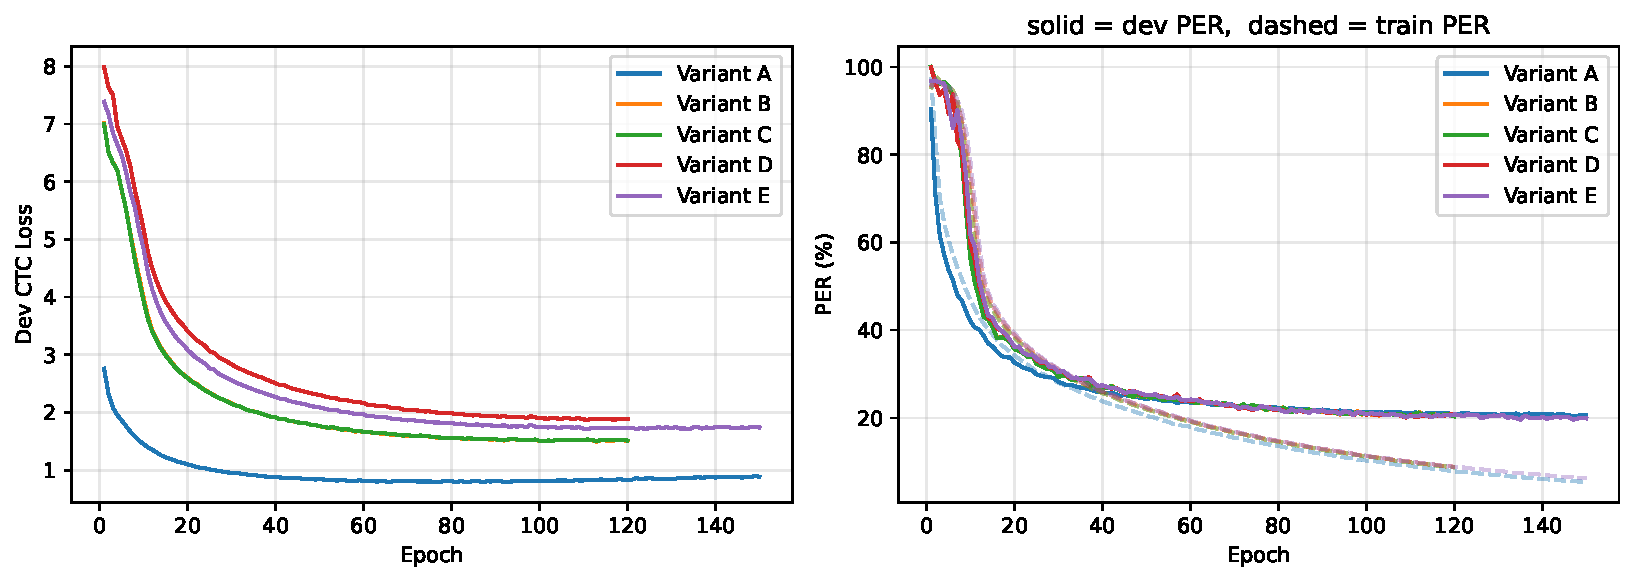
\includegraphics[width=\linewidth]{../experiments/training_curves.pdf}
\caption{Dev CTC loss (left) and PER curves (right) for all variants.
  Solid lines: dev PER; dashed lines: train PER.  Variant E (full model)
  reaches the lowest final dev PER.}
\label{fig:training}
\end{figure}

\subsection{Sanity Check: A@150 Epochs}

A critical confound is that Variant E trains for 150 epochs while Variant
A trains for only 80.  We re-trained Variant A for 150 epochs
(matched budget) and observed \textbf{20.48\% PER} --- identical to the
80-epoch result.  This confirms that the gain of E over A is attributable
to the objective, not the additional training budget.

\subsection{Hyperparameter Ablations}

\paragraph{Smoothness weight $\lambda$.}
Figure~\ref{fig:lambda} shows the effect of $\lambda$ on PER for Variants
C and E.  For Variant C, PER is nearly flat across $\lambda\in
\{10^{-3},5\times10^{-3},10^{-2}\}$ (20.36--20.45\%), indicating that
smoothness alone is not strongly tunable on this acoustic head.  For
Variant E, $\lambda=5\times10^{-3}$ yields the best result (19.75\%).
The complementarity of skip-diphone and smoothness is evidenced by the
strictly lower PER of E versus C at all $\lambda$ values.

\begin{figure}[h]
\centering
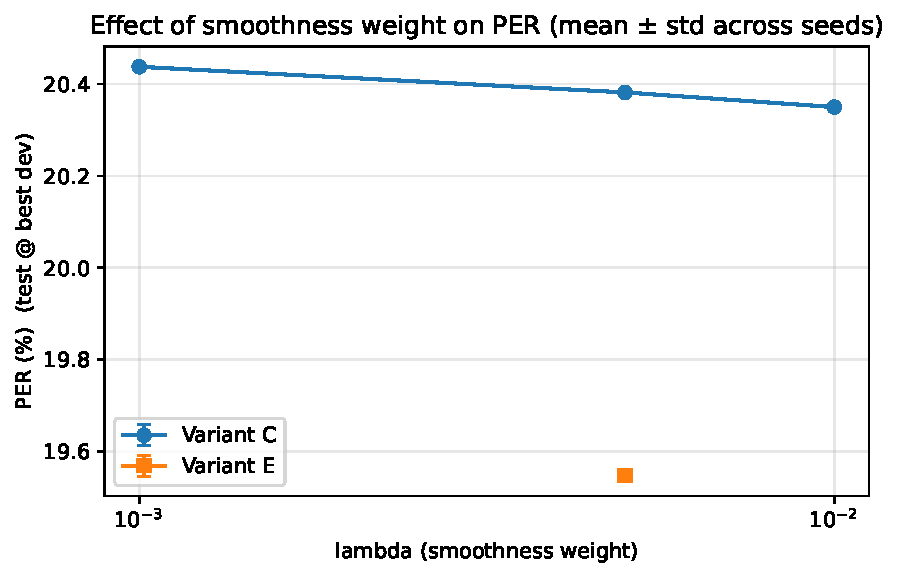
\includegraphics[width=0.9\linewidth]{../experiments/lambda_sweep.pdf}
\caption{Effect of smoothness weight $\lambda$ on test PER for Variants
  C and E.  E consistently outperforms C, demonstrating that the
  skip-diphone and smoothness objectives are complementary.}
\label{fig:lambda}
\end{figure}

\paragraph{Skip-diphone weight $\beta$.}
Figure~\ref{fig:beta} shows Variant D's PER across
$\beta\in\{0.05,0.1,0.2,0.3\}$.  The optimum is at $\beta=0.2$ (20.12\%
PER); $\beta=0.3$ degrades sharply to 20.47\%, suggesting that an
excessively strong auxiliary loss disrupts the primary diphone CTC
objective.

\begin{figure}[h]
\centering
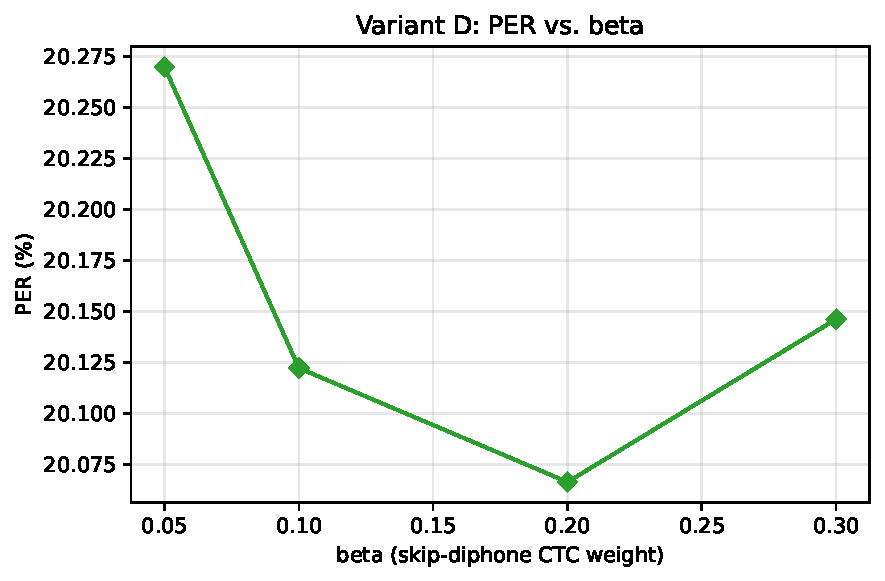
\includegraphics[width=0.9\linewidth]{../experiments/beta_sweep.pdf}
\caption{Variant D: PER vs.\ skip-diphone weight $\beta$.  The optimum
  is at $\beta=0.2$; larger $\beta$ overpowers the primary diphone CTC
  loss.}
\label{fig:beta}
\end{figure}

\subsection{WER Analysis}

Table~\ref{tab:ablation} and Figure~\ref{fig:heatmap} show the WFST
decoding results.  Variant E achieves the best 5-gram WER among diphone
models (18.56\%), but Variant A wins overall (18.07\%).  Two empirical
observations characterize the PER--WER gap:

\textbf{1. Skip-diphone hurts WER.}  All four D variants land at
20.05--20.41\% 3-gram WER, roughly 0.8--1.2 pp worse than B (19.23\%),
despite D having better PER.  We \emph{hypothesize} that the skip-diphone
auxiliary loss pushes the encoder to encode longer-range context, which
improves the per-frame phone \texttt{argmax} that PER measures but smears
the blank/phone temporal structure that the WFST decoder relies on to place
boundaries.  This is consistent with the data but not directly established:
we can rule out a pure marginalization artefact (B/C share the same
marginalization without the regression), but not a calibration mismatch or
an under-resolved $(ac, bp)$ grid.  A direct test---comparing blank-spike
sharpness or forced-alignment entropy across variants, or re-decoding
temperature-rescaled skip posteriors---is left to future work.

\textbf{2. Smoothness helps WER among the diphone variants.}  Variant C
($\lambda=0.005$) attains the best 3-gram WER of any diphone variant
(19.01\%), beating B by 0.22 pp.  It does not, however, beat the monophone
baseline: A measured 19.00\%, and since A's sweep used a narrower grid whose
blank-penalty curve was still declining, that figure is an \emph{upper bound}
on A's 3-gram minimum.  A and C are therefore not separated by this
experiment.  Temporally smoother phone posteriors do appear to produce
cleaner CTC lattices relative to the unsmoothed diphone model.

\textbf{3. Calibration mismatch.}  Diphone marginalization (log-sum-exp
over 40 contexts) yields a softer, higher-entropy phone distribution than
direct monophone CTC.  The WFST decoder, calibrated for monophone-CTC
spike trains, requires a higher blank penalty to compensate (Variant E:
$\text{bp}=7$ vs.\ A: $\text{bp}=4$ on 5-gram).  This recalibration cost
is amplified by the strong 5-gram LM, which further dilutes the acoustic
contribution.

\begin{figure}[h]
\centering
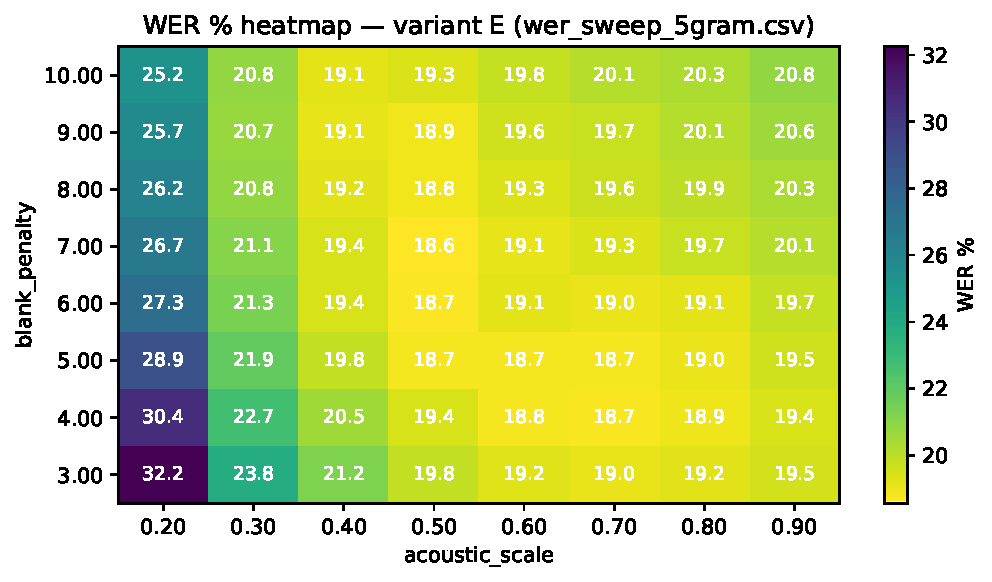
\includegraphics[width=\linewidth]{../experiments/wer_heatmap.pdf}
\caption{WER (\%) heatmap for Variant E (5-gram sweep).  The optimal
  cell is $(\text{ac}=0.5, \text{bp}=7.0)$, reflecting the higher blank
  penalty required by the diphone model compared to the monophone baseline.}
\label{fig:heatmap}
\end{figure}

% ---------------------------------------------------------------
\section{Conclusion}

We presented two acoustic-model extensions of DCoND for intracortical
speech BCI: a skip-diphone auxiliary CTC head and a temporal smoothness
regularizer.  The full model (Variant E) achieves 19.75\% PER on the
Brain-to-Text '24 benchmark, a 0.73 pp absolute reduction (3.6\% relative)
from the monophone CTC baseline (20.48\%).  A matched-budget sanity check
confirms that this gain reflects the objective, not training time.

Honest analysis reveals that PER improvements do not transfer to WER under
WFST-only decoding: the monophone baseline (A) retains the best 5-gram WER
outright (18.07\% vs.\ E's 18.56\%) and is at least tied with the best diphone
variant on 3-gram (A $\leq$19.00\% vs.\ C's 19.01\%), with smoothness-only (C)
the strongest of the diphone variants there.  The
most likely mechanism is a calibration mismatch introduced by diphone
marginalization; we further hypothesize a contribution from the skip-diphone
head perturbing blank/phone temporal structure, though this is not directly
measured here and remains to be tested.

Future work should explore (i) GPT-2 n-best rescoring as in DCoND, which
is complementary to our acoustic objective and may recover the WER gap;
(ii) a diphone-aware WFST or RNN-T decoder that avoids marginalization;
and (iii) modifications to the skip-diphone head to preserve blank/phone
temporal calibration while retaining the articulatory context benefit.

% ---------------------------------------------------------------
\bibliographystyle{plain}
\bibliography{report}

\end{document}
